\section{Introduction}

I have yet to see any problem, however complicated, which, when looked at in the right way did not become still more complicated.

\begin{flushright}--- Poul Anderson\end{flushright}

People working in the field of high energy physics have a tendency to concern themselves with attempting to solve problems that are incredibly complicated.
So, perhaps, there is a touch of irony that the problem that they are trying to solve is not only incredibly fundamental, but also very simple to state.
The question can be boiled down to -- what is the stuff in our universe made of?
What immediately follows from this fundamental inquiry is - how is matter made up of these things? Or to put it another way, how do the fundamental building blocks interact?

In some sense, particle physics tries to distill matter and the interactions therein down to the smallest possible level to which it can be broken down.
Turns out that breaking these concepts down to this elementary level of specificity is an incredibly complicated process of which we have merely begun to scratch the surface.  As such, this paper focuses on a tiny fraction of these fundamental building blocks -- the elusive neutrino with the hope of just perhaps being able to untangle some of the myriad of secrets that it harbours.

\subsection{The Standard Model}

Before the protagonist
\footnote{Really the ensemble cast, given that they come in three flavors, electron($e\nu$), muon ($\mu \nu$) and tau($\tau \nu$)and their respective antiparticles,}
of our story - the neutrino - can be formally introduced, the stage has to be set.
A good candidate to set the stage would be the standard model which describes three of the four known fundamental forces, electromagnetic, weak and strong interactions (it struggles to deal with  gravity) and classifying all known elementary particles \cite{Oerter}.
Just like any foundational theory that undergirds a sub-field of a subject, the standard model definitely wasn't developed in a day and as such, there is definite value in becoming familliar with the historical context surrounding the standard model in our quest to understand neutrinos.

One may definitely quibble about where our understanding of the fundamental particles starts from, after all, humans have been trying to find out the nature of our universe and the things that make it up going back as far as the 4th century BCE with Plato positing that everything is made up of 4 elements (water, wind, earth and fire)\cite{Timaeus}, but I think it makes sense to look at the elementary particles that make up the standard model as we know it today -- with the definite understanding that there may very well be physics that lies beyond the realm of the standard model.

At its core, the Standard Model consists of two main categories of particles: fermions, which make up matter, and bosons, which mediate interactions.
Fermions have $1/2$ integer spins while bosons have integer spins \cite{Oerter}.

\begin{figure}[H]
  % 
  \centering
  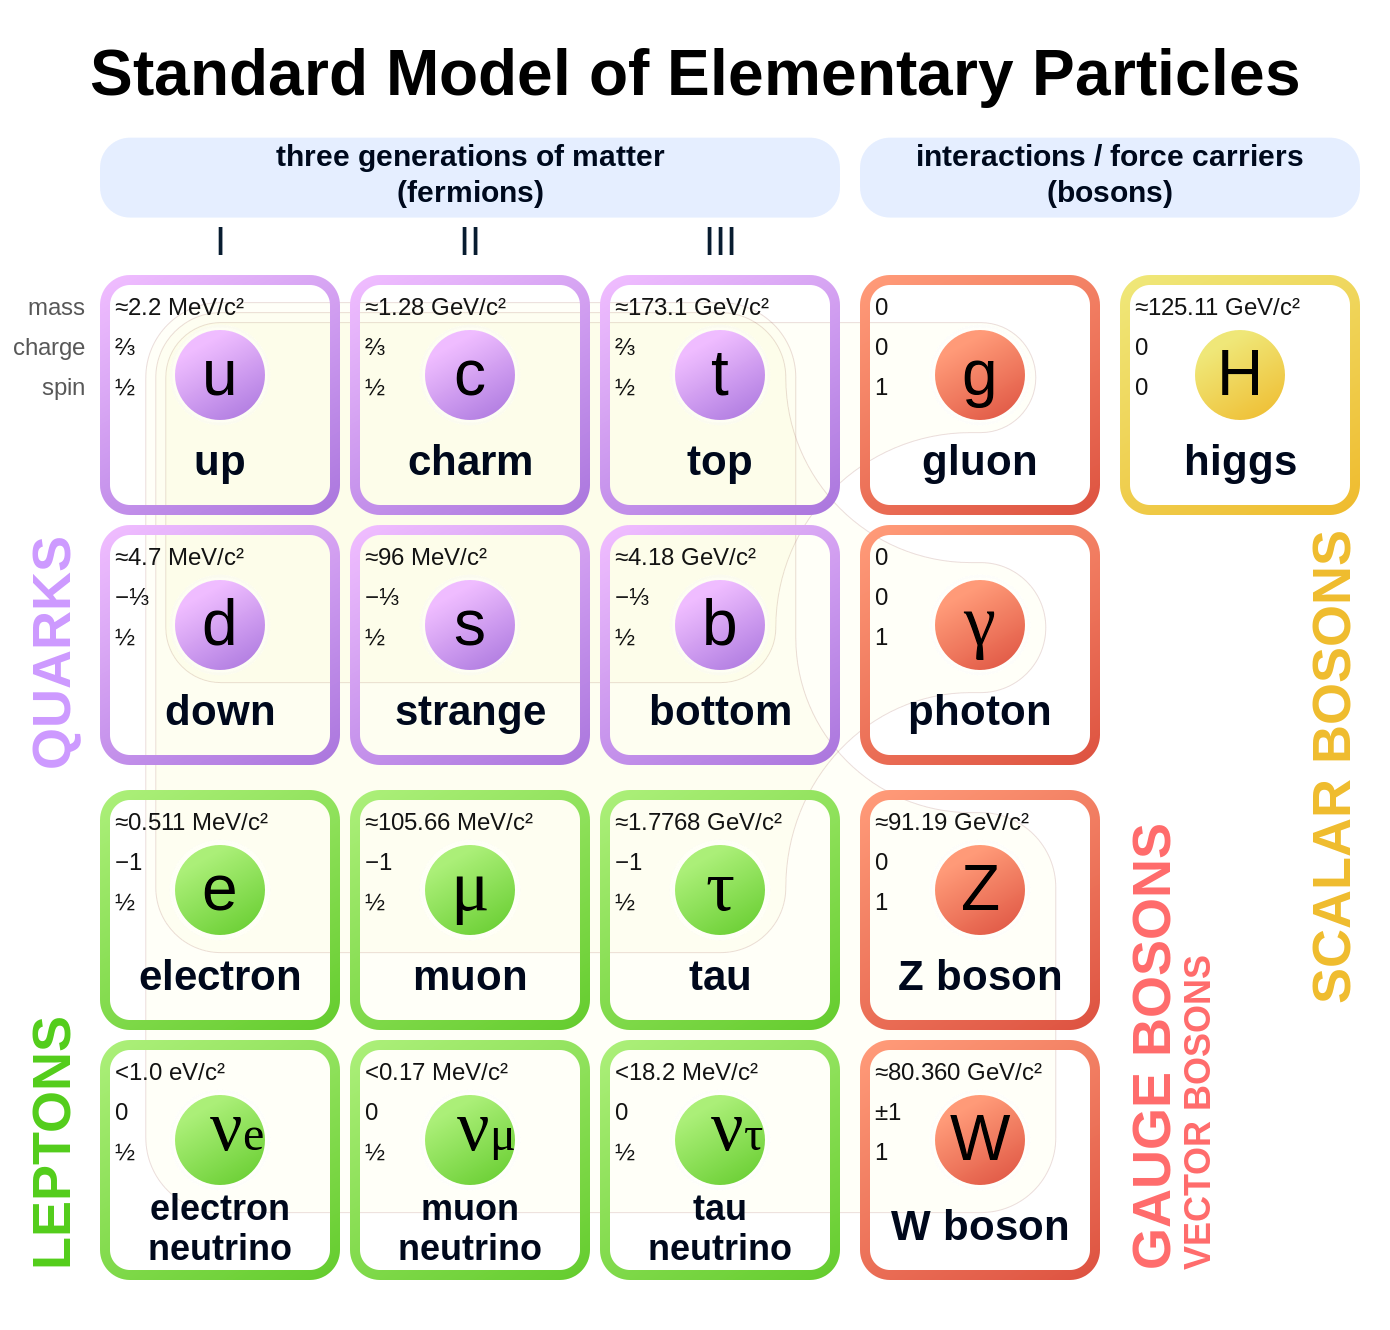
\includegraphics[width=80mm]{figures/sm.png}
  \caption{The Elementary Particles in the Standard Model \cite{standard_model}}
  \label{sm}
\end{figure}

The fermions can be further categorized into quarks and leptons.

\begin{figure}[H]
  % https://en.wikipedia.org/wiki/Quark#/media/File:Quark_structure_proton.svg
  \centering
  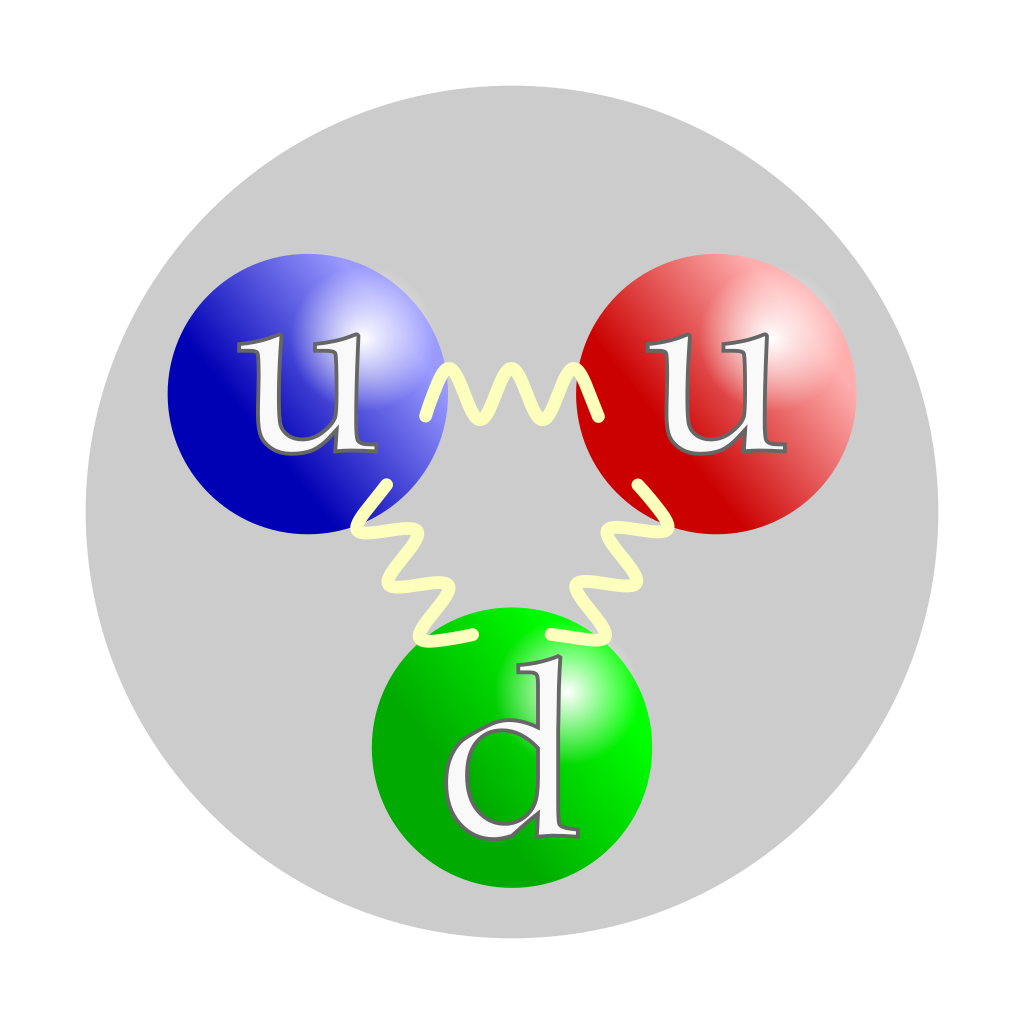
\includegraphics[width=100mm]{figures/protonQuarks.png}
  \caption{Quarks inside a proton.
    Labelled u for up and d for down\cite{quark}}
  \label{protonQuarks}
\end{figure}

Quarks are understood to be fundamental constituents of matter, forming the building blocks of protons, neutrons, and other hadrons (Composite subatomic particles that are made up of at least 2 quarks) \cite{quark_Brit_2024}.
Quarks interact with each other via the strong force.We have so far discovered 6 flavors of quarks -- up (\(u\)), down (\(d\)), charm (\(c\)), strange (\(s\)), top (\(t\)), and bottom (\(b\)).
Each flavor has different mass.
These masses and their interactions with other particles are crucial for the stability and properties of atomic nuclei \cite{Nave_quark}.

\begin{table}[h!]

  \centering
  \begin{tabular}{lrr}
    \toprule
    Quark Flavor & Approximate Mass (MeV/c\(^2\)) & Charge (e) \\
    \midrule
    Up (u)      & 2.2 - 3.0        & +\(\frac{2}{3}\) \\
    Down (d)    & 4.7 - 5.0        & -\(\frac{1}{3}\) \\
    Strange (s) & 95 - 105         & -\(\frac{1}{3}\) \\
    Charm (c)   & 1270 - 1720      & +\(\frac{2}{3}\) \\
    Bottom (b)  & 4180 - 4380      & -\(\frac{1}{3}\) \\
    Top (t)     & 172000 - 173000  & +\(\frac{2}{3}\) \\
    \bottomrule
  \end{tabular}
  \caption{Quark Flavors, Their Approximate Masses and Charges \cite{Nave_quark}}
  \label{quarkMass}
\end{table}

Each type of fermion carries a specific flavor and generation.
For instance, the electron ($e$) belongs to the first generation, while the muon ($\mu$) and tau ($\tau$) belong to the second and third generations, respectively \cite{Nave_lepton} \footnote{The neutrino, despite being elusive, plays a significant role in weak interactions and lepton family conservation.}.

The interactions between these particles are mediated by gauge bosons, which are the force carriers \cite{Gribbin_2000}\cite{Clark_2004}.
The Standard Model includes the following gauge bosons:

\begin{align}
 & \quad \text{Photon } (\gamma) \quad \text{(mediates electromagnetic force)} \\
                    & \quad \text{W and Z bosons } (W^\pm, Z^0) \quad \text{(mediates weak force)} \\
                    & \quad \text{Gluons } (g) \quad \text{(mediates strong force) \cite{Veltman_2004}}
\end{align}

The mathematical framework underpinning the Standard Model is primarily based on gauge theory, specifically the group $SU(3) \times SU(2) \times U(1)$.
Each of these groups corresponds to a different force:

\begin{align}
\text{Strong Interaction:} & \quad SU(3) \quad \text{(color charge)} \\
\text{Weak Interaction:} & \quad SU(2) \quad \text{(isospin)} \\
\text{Electromagnetic Interaction:} & \quad U(1) \quad \text{(hypercharge)}
\end{align}

The Higgs mechanism, a crucial part of the Standard Model, provides a mass to the W and Z bosons via spontaneous symmetry breaking.
The Higgs field $\phi$ can be parameterized as:

\begin{align}
\phi &= \frac{v+h}{\sqrt{2}}e^i{\frac{\chi}{v}}
\end{align}

where $h$, the Higgs boson and $\chi$, the Goldstone boson are real scalar fields which have no vacuum expectation value.
The mass terms for the gauge bosons arise when the Higgs field acquires a vacuum expectation value\cite{Bernardi_2008}.



% \subsection{The Electron}

For the longest time, humans had thought that atoms were the smallest particle that makes up everything in the world and cannot be subdivided further\cite{Dalton}, but this idea had started to come under scrutiny by the late 1800's\cite{Pullman}.
Even then, it was thought that if anything were to make up atoms, they wouldn't be lighter than the lightest atom \cite{Thorpe}.
However, in 1897, Thomson would come in with evidence that there not only were particles that made up the atoms, but that they were on the scale of 1000 times lighter than hydrogen\cite{Thomson_1907}.
He decided to shoot cathode rays at a thermal junction so he could measure the generated heat and measured how much they deflected magnetically.
He also measured the electrical deflections by lowering the pressure in the chamber where he was measuring the deflection\cite{Thomson}.
Through these experiments, he discovered the electron
\footnote{Although Thomson did decide to call them corpuscles; a name which definitely did not stick around}
and believed that it was a fundamental part of all atoms that was very light and held a decidedly negative charge\cite{electronDiscovery}.



% \subsection{Models of the Atom}

The discovery of something so much smaller than the lightest atom threw Dalton's atomic theory out the window.
His theory claimed that  everything in the universe was made up of atoms which would vary in size and mass based on the element.
These atoms could not be created or destroyed, but  could reaarrange themselves through chemical reactions.
It could be argued that Dalton's model was a progenitor for the idea of conservation of mass and energy.
Despite being such an important idea, even before the discovery of electrons, the theory wasn't fullproof; it could not account for isotopes of the same element having different masses, but the electron blew the idea wide apart.

A new theory that looked at the atom not as the smallest thing that could exist but rather something that had other things inside in some sort of structure had to be developed.

There were numerous models that tried to tackle this problem and one of the first was proposed by Thompson in 1904 as the plum pudding model.
The first problem to grapple with was that electrons are negatively charged while the atoms themselves are electrically neutral.
To get around this, the plum pudding model suggests that  the electrons were suspended in a morass of positively charged particles
\footnote{Kind of like plums suspended in a pudding, hence the name of the model}
with the charge between the positive  and negative equalling out to 0.
Thomson believed that the mass was evenly distributed throughout the atom.

\begin{figure}[H]
  % https://en.m.wikipedia.org/wiki/File:Plum_pudding_atom.svg
  \centering
  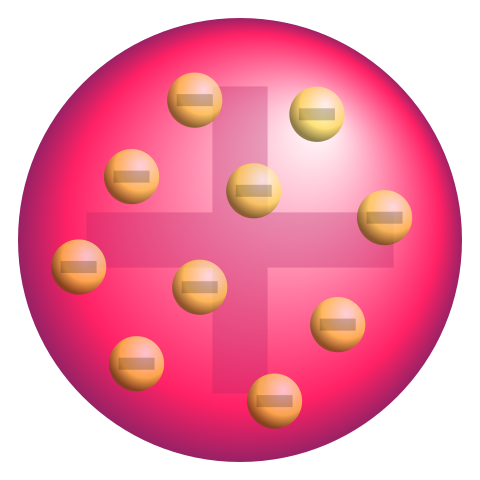
\includegraphics[width=100mm]{figures/plumPudding.png}
  \caption{Cartoon of plum pudding model}
  \label{plumPudding}
\end{figure}

The plum pudding model struggled to explain how these charged particles were so copacetic with each other despite being such small physical distances apart.
It was well known by then that opposite charges attract while alike charges repel.
It also failed to provide any explanation of the spectral lines observed in hydrogen.
Darker clouds were still on the horizon for Thomson's plum pudding model.

Between 1908 and  1913, a number of alpha ($\alpha$) particle scattering experiments were performed by Hans Geiger and Ernest Marsden.
These took the form of shooting $\alpha$  particles at a  incredibly thin piece of gold foil.
Based on the plum pudding model, it was expected that the $\alpha$ particles would not be deflected however this turned out not to be the case at all.
To be fair, most of the $\alpha$ particles did indeed go straight through the gold foil, their trajectory not disturbed in the slightest.
A smaller fraction did get deflected, some by a small angle and others by a large one.
But the astonishing part was that an even smaller fraction, about 1 in 20000, shot right back at the direction the particle gun was shooting from.

\begin{figure}[H]
  % https://en.wikipedia.org/wiki/Rutherford_scattering_experiments#/media/File:Geiger-Marsden_experiment_expectation_and_result.svg
  \centering
  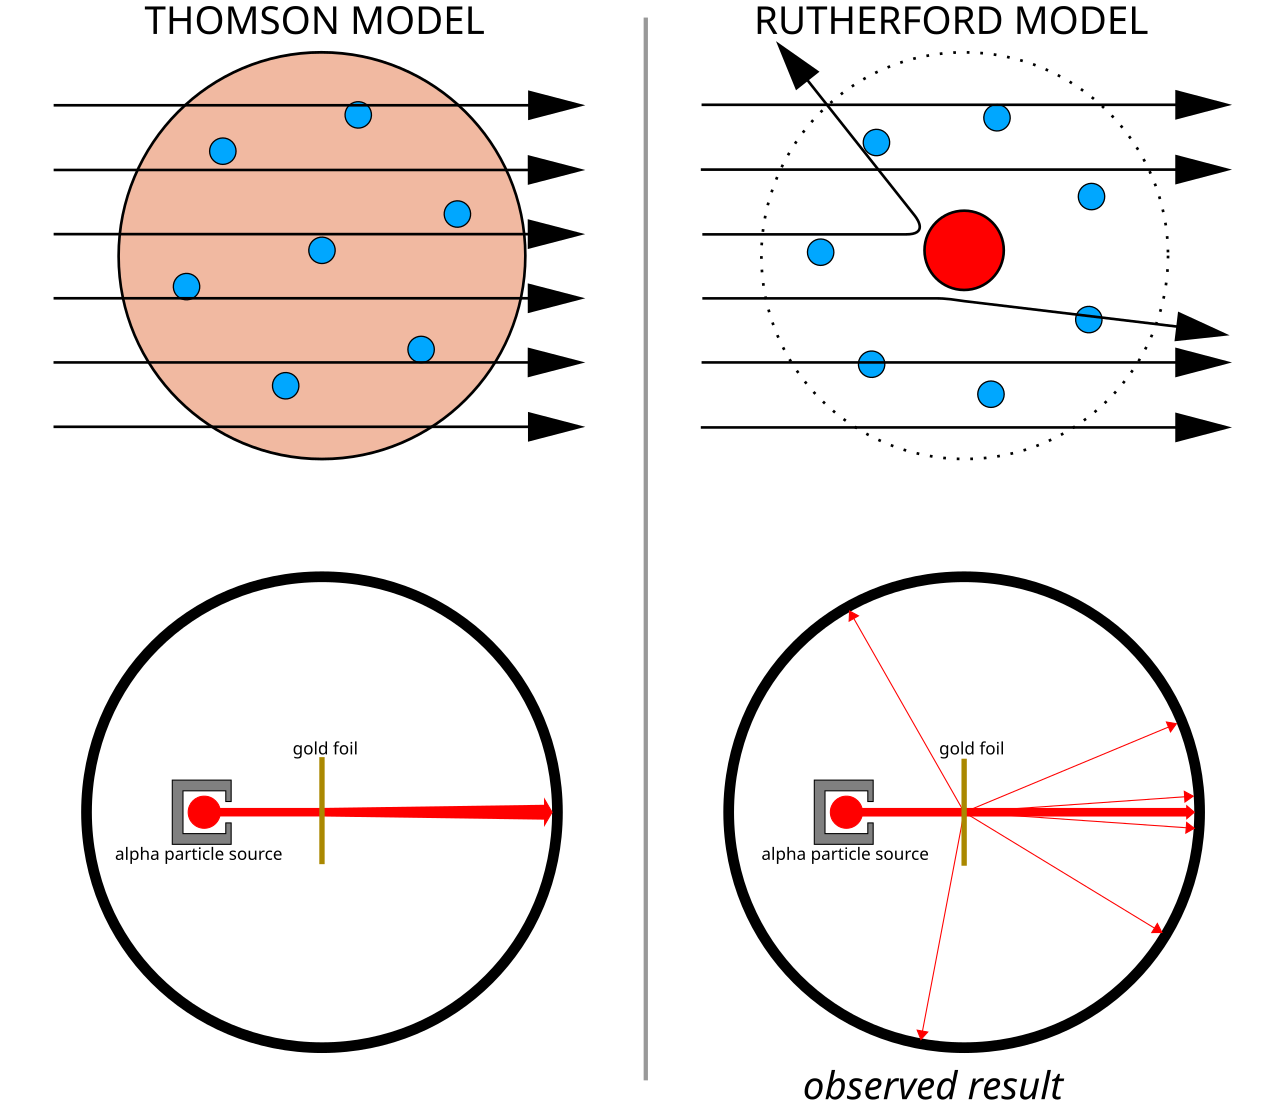
\includegraphics[width=100mm]{figures/goldFoil.png}
  \caption{Cartoon of Gold foil experiment}
  \label{goldFoil}
\end{figure}

So a new model was required to explain the discrepencies away; in comes Rutherford.
He looked at the gold foil experiments done before him and ran with it, expanding upon them and developing a new theory on the substructure of the atom.
He proposed in 1911 that atoms were mostly just empty spacewith a highly concentrated segment of mass at the center of the atom -- he called this central mass the neucleus of the atom.
In Rutherford's atomic model, the electrons orbit around the positively charged neucleus.

\begin{figure}[H]
  % https://en.wikipedia.org/wiki/Rutherford_model#/media/File:Rutherford_atomic_planetary_model.svg
  \centering
  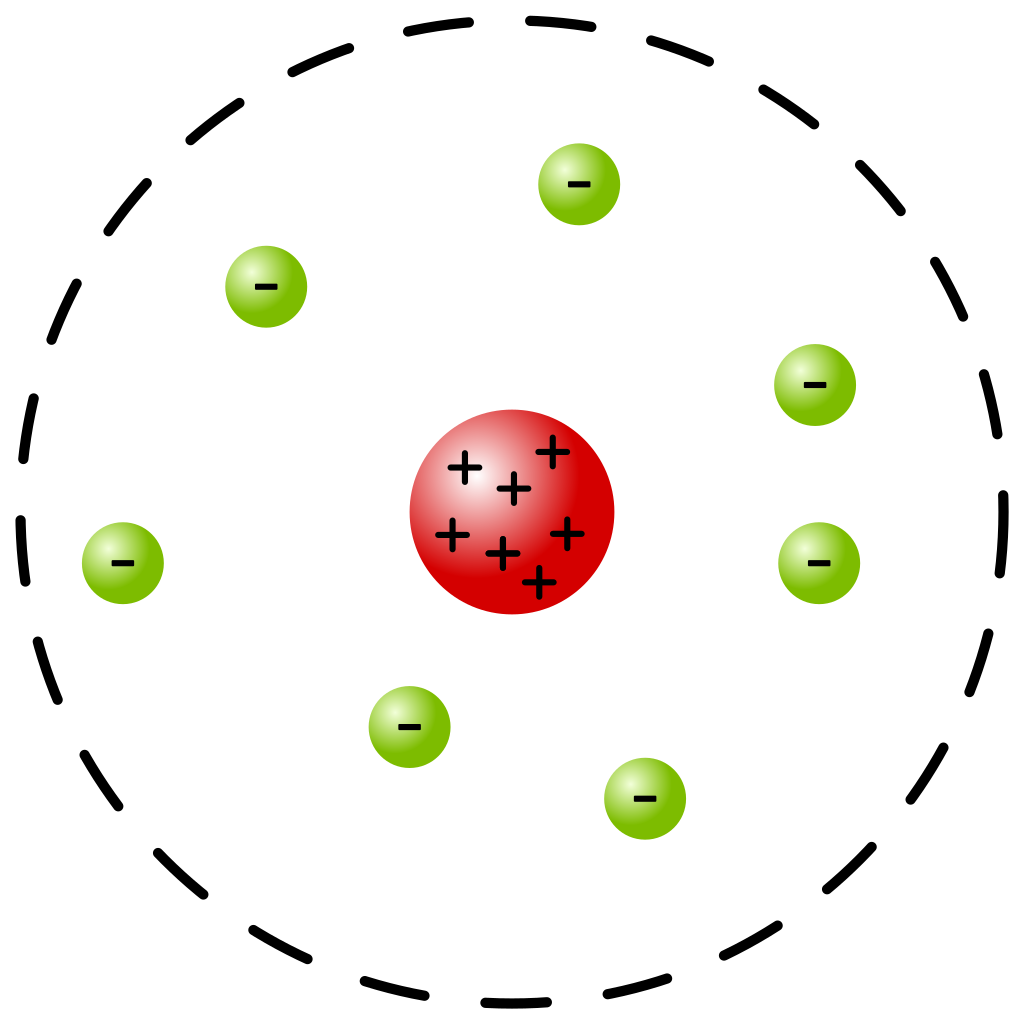
\includegraphics[width=100mm]{figures/rutherford.png}
  \caption{Rutherford's atomic model}
  \label{rutherford}
\end{figure}

Only, one little problem.
When things move in a circular orbit, they are accelerating and when a charged particle is moving in an orbit like that,  it should be constantly radiating energy leading to it eventually falling into the neucleus rendering this formulation of the atom unstable.
It should also be emitting a continous energy spectrum from the electrons, but hydrogen has discrete spectral lines.

Bohr tried to come at this from an angle that resolved the spectral line issue with Rutherford's model.
Bohr proposed that electrons move in fixed orbits, thus explaining the discrete lines of the hydrogen spectra and that atoms emit light when an electron jumps from a higher energy level to a lower one.

\begin{figure}[H]
  % https://en.wikipedia.org/wiki/Bohr_model#/media/File:Bohr_atom_model.svg 
  \centering
  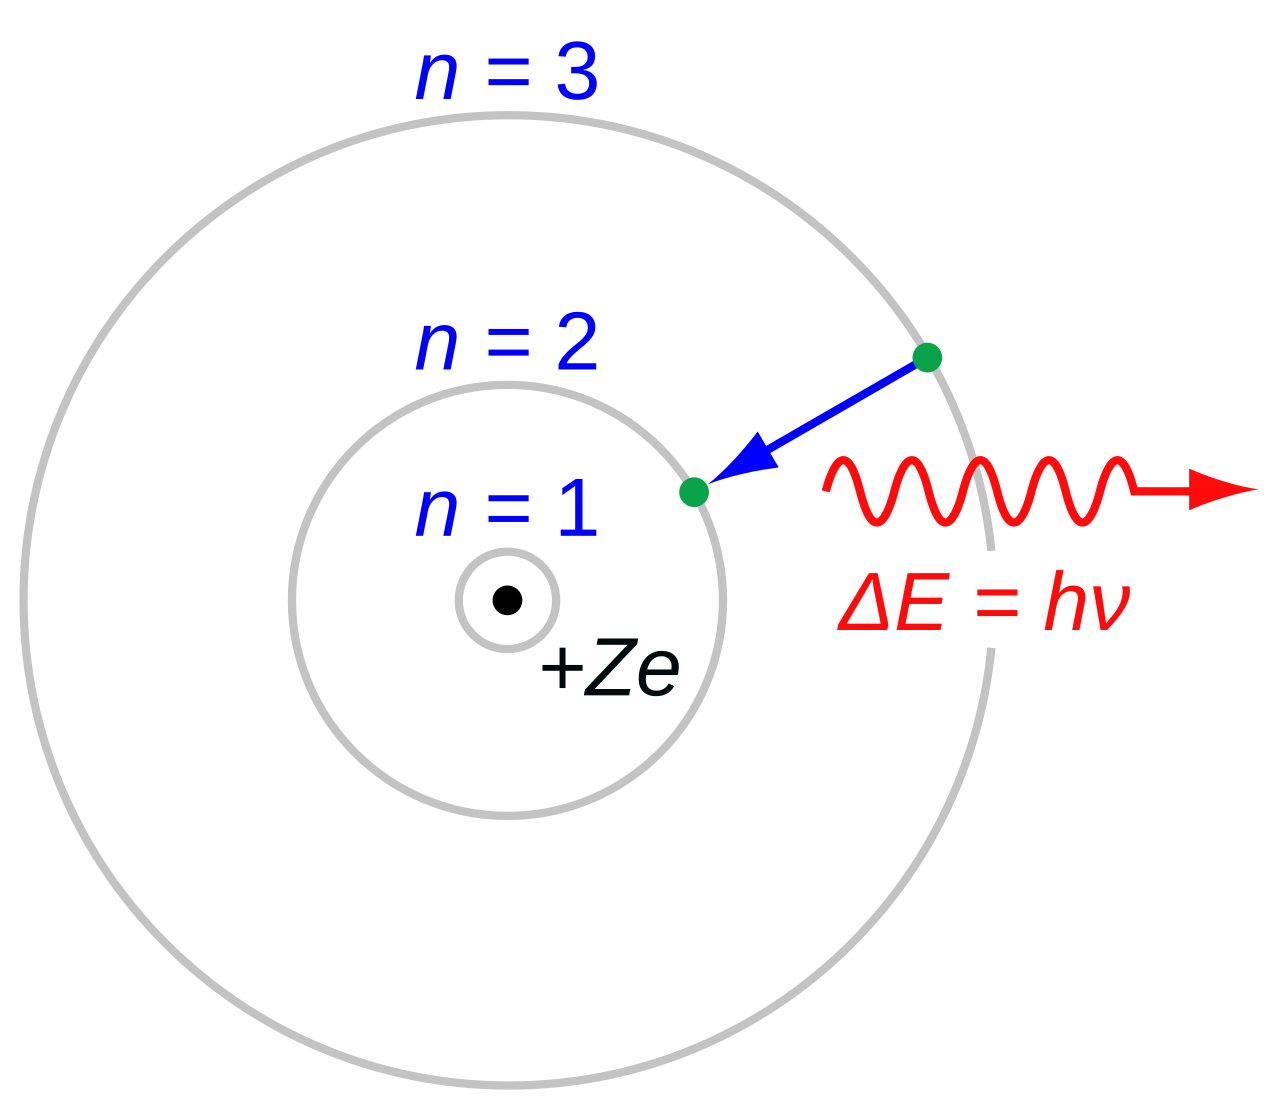
\includegraphics[width=100mm]{figures/bohr.png}
  \caption{Bohr's model of the hydrogen atom}
  \label{bohr}
\end{figure}

This still doesn't explain away why the electron doesn't collapse into the neucleus .
However, it does a very good job of modelling hydrogen and hydrogen-like atoms under most normal conditions.
The other issue with Bohr's model is that it fails to adress De-Broglie’s Hypothesis of the dual nature of matter..
To get there, we have to delve into the wonderful world of quantum mechanics.


% \subsection{The Photon}

What led to the development of quantum mechanics was spirited debate about the true nature of light.
Newton was one of the first to throw his hat into the ring; in 1672 he decided to build upon the corpuscular theory coined by Descartes, arguing that light was made up of discrete particles just like everything else.
Problem was, that around the same time Robert Hooke and Christian Huygens performed experiments  that led them to believe light was in fact not a stream of particles but rather a wave.
This wave view of light did a much better job of explaining how light refracted compared to Newtons model.

The position of people beliving that light was in fact a wave, not particles got a lot stronger in 1801 thanks to double slit experiments by Thomas Young.
This was an experiment where there were two slits cut into a screen and light was then shone through it being visible on another screen once it had made it past the slits.
If light was indeed made up of particles, the expectation was that we would see essentially 2 bright spots on the final screenthat corresponded to the two slits.
Instead, what we got was an interference pattern that iss typical of waves.

\begin{figure}[H]
  % https://en.wikipedia.org/wiki/Double-slit_experiment#/media/File:Double-slit.svg
  \centering
  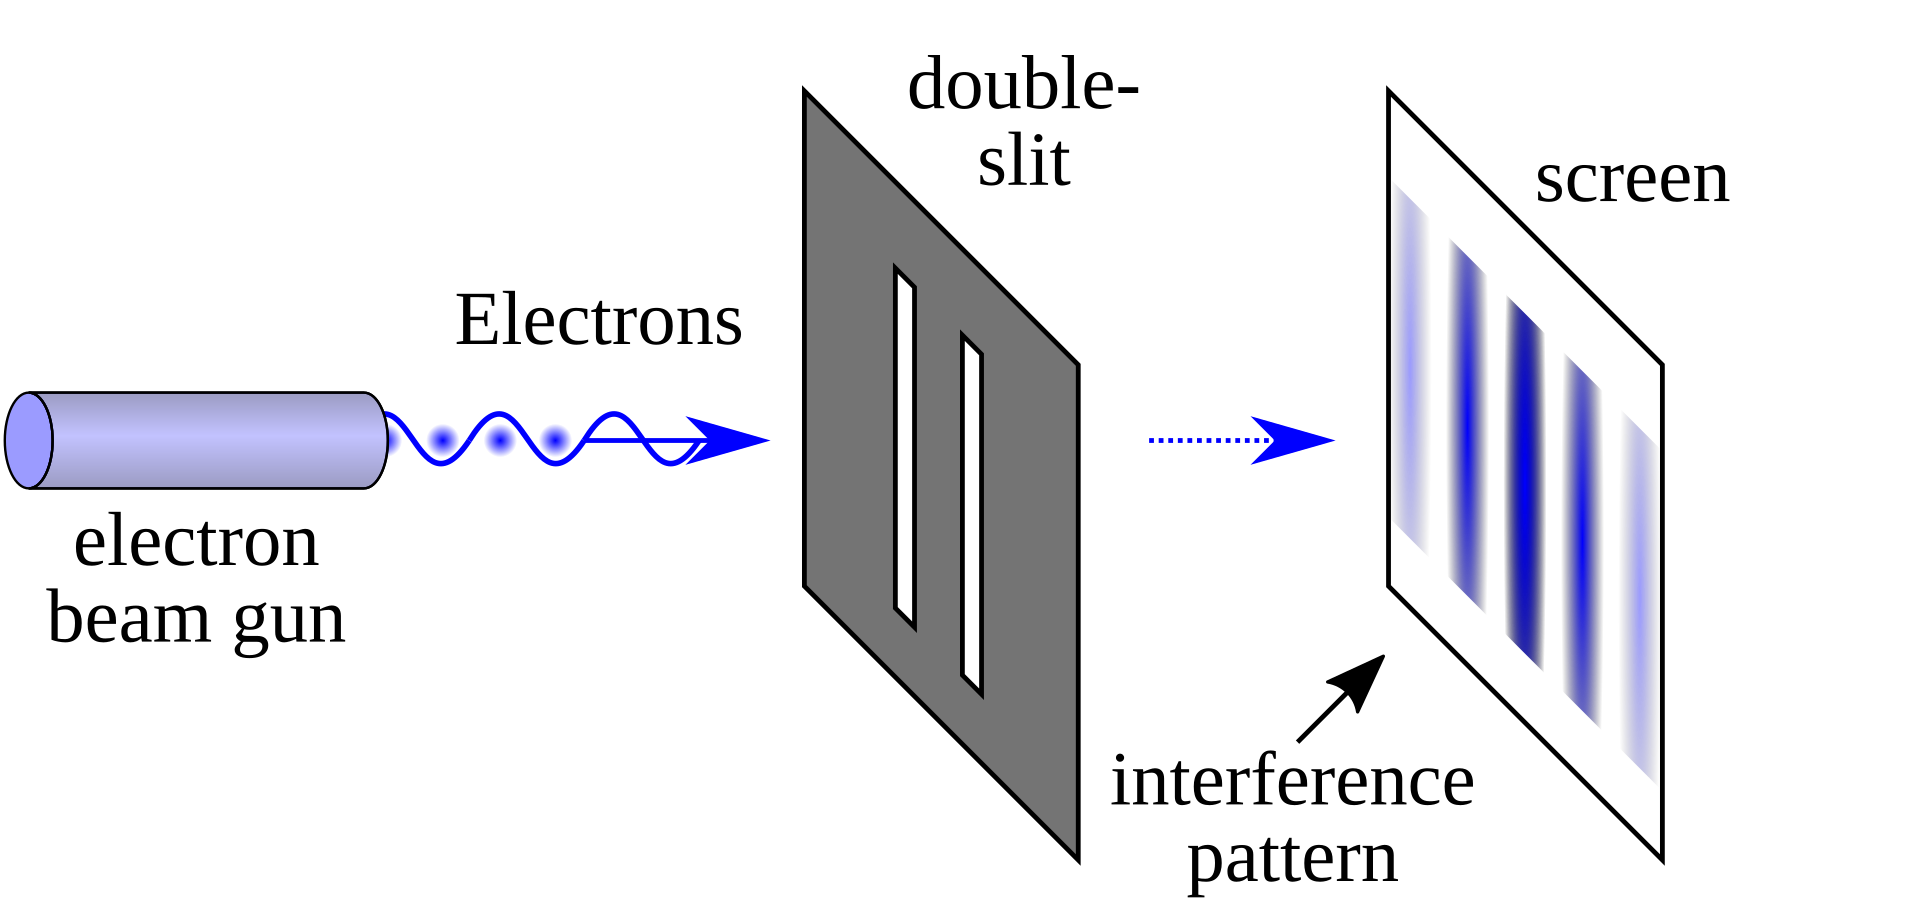
\includegraphics[width=130mm]{figures/doubleSlit.png}
  \caption{Double Slit Experiment}
  \label{doubleSlit}
\end{figure}

At this point, the world is pretty much in the wave camp for the purposes of modelling light, but the idea that light is made of particles was about to be revived from the dead by none other than Max Planck.
He was trying to solve the problem of black body radiation; namely, that the energy carried by electromagnetic waves is emitted and absorbed in discrete quantities.
His solution was to  come up with the idea of discrete quanta rather than a continously emmisive spectrum.
He did this through the creation of the what we call the Planck constant today ($h$), a proportionality constant  that he called  the quantum of action.

This was fundamentally the introduction of quantum mechanics.  a quite contentious idea at the time, highlighted by the following quote from Bohr.

quantum theory cannot possibly have understood it.

\begin{flushright}--- Neils Bohr\end{flushright}

Despite being frought in debate, the idea of quantum mechanics simply would not go away.
Einstein would go on to build on the Planck's ideas and proposed that light was made up of discrete packets of energy that he called photons.
He developed the Planck-Einstein Relationship, connecting  energy and the frequency of light.

\begin{align}
  E = h \nu
\end{align}

Where $E$ stands for energy, $h$ for thePlanck constant and $\nu$ for the frequency of the photon.

% Could you please check if the equation is correct, I'm not totally sure about the \nu

This equation was to explain the results that Einstein had gotten from his experiments regarding the photoelectric effect.
In 1914, Robert A. Millikan went on to confirm Einstein's idea by doing  a highly accurate measurement of Plank's Constant  using the photoelectric effect.
Photons would go on to be included in the list of particles we deal with in the standard model today.





% \subsection{Duality of Matter}This new evidence went in the face of the wave nature of light which had been longstanding.
It seemed like  there were phenomena that could be explained by thinking of light as a wave and other phenomena that could be understood if we looked at light as a particle.
In 1924, Louis de Broglie entered the fray and decided to ask the question nobody had before.

But why not both?

He even went a step further and argued that the wave/particle dual nature was not just a thing for light, but rather all matter.

He further worked on Einstein's equation, ending up with

\begin{align}
  h \nu_0 = m_0 c^2
\end{align}

Where $h$ is the Planck constant, $\nu_0$ is the frequency, $m_0$ is the mass while $c$ is the speed of light in a vaccum. Leading to Einstein's famous equation

\begin{align}
  E = m c^2
\end{align}

Where $E$ is energy, $m$ is mass and $c$ is the speed of light in a vaccum.

This work led to the De Broglie's relationship between wavelength and momentum.

\begin{align}
  \lambda = \frac{h}{p}  
\end{align}

Where $\lambda$ means wavelength, $h$ is the Planck constant and $p$ is momentum.

This relationship can be thought of as a particle travelling through space as a wave packet.
This hypothesis was later confirmed through cathode ray diffraction and Davison-Germer experiment.

Erwin Schrödinger would go on to take the ideas developed by De Broglie and run with it.
He thought that if all matter can be thought of as a wave packet, there must be a wave equation to describe them.
Thus the  Schrödinger's equation was born.

\begin{align}
  i \hbar \frac{\partial \Psi(\mathbf{r}, t)}{\partial t} &= \left[ -\frac{\hbar^2}{2m} \nabla^2 + V(\mathbf{r}, t) \right] \Psi(\mathbf{r}, t) 
\end{align}

Where
\begin{itemize}
\item $\Psi(\mathbf{r}, t)$ stands for the wave function of the quantum system, which depends on both position $\mathbf{r}$ and time $t$.
\item $i$ is the imaginary unit.
\item $\hbar$ is the reduced Planck constant.
\item $\frac{\partial \Psi(\mathbf{r}, t)}{\partial t}$ denotes the partial derivative of the wave function with respect to time.
\item $\nabla^2$ is the Laplacian operator, representing the sum of second partial derivatives with respect to the spatial coordinates, indicating the kinetic energy term.
\item $V(\mathbf{r}, t)$ is the potential energy of the system, which may vary with position and time.
\end{itemize}

% \subsection{Electron Cloud Model}

The Schrödinger's equation would pave the way for the electron cloud model of the atom we use today, but there has to be a little more work to be done befpore we can get there.
The next step in the journey relates to Heisenberg and his famous uncertainity principle.
In his model of the atom, he  never explicitly talked about the physical position or momentum of the electron; definitely breaking with tradition. Instead, his theory focused on the observables of the electron, namely the frequency of light emitted or absorbed. He would go on to refine his uncertainity principle to state

One can never know with perfect accuracy both of those two important factors which determine the movement of one of the smallest particles—its position and its velocity (or momentum). It is impossible to accurately determine both the position and velocity of a particle at the same instant.

\begin{flushright}--- Werner Heisenberg,\end{flushright}

Or to present the idea in math form,

\begin{align}
  \Delta x \cdot \Delta p &\geq \frac{\hbar}{2} \\
  \Delta E \cdot \Delta t &\geq \frac{\hbar}{2}
\end{align}

Where $\Delta x$ stands for the uncertainty in position, $\Delta p$ stands for the uncertainty in momentum, $\Delta E$ stands for the uncertainty in energy, and $\Delta t$ stands for the uncertainty in time. $\hbar$ represents the reduced Planck constant.

% \subsection{Protons and Neutrons}

We have looked a lot at the structure of the atom and what surrounds the nucleus, but what exactly does the nucleus contain?
To do that, we have to go back in time a little bit.

In the early 20th century, it was understood that the nucleus, as proposed by Rutherford, was a dense central core of the atom.
However, this model did not fully explain the mass of the nucleus nor the nature of its internal components.
In 1917, Ernest Rutherford made a significant contribution by identifying the proton.
His experiments with alpha particles bombarding nitrogen gas led to the discovery of a new particle.
This was a positively charged particle in the center of the nucleus; What we call the proton today.

Despite Rutherford's discovery of the proton, there remained a critical question: if the nucleus contained protons, why did it not have enough charge to account for the total mass of the atom? This discrepancy led to the hypothesis of the neutron, a neutral particle within the nucleus.

In 1932, James Chadwick provided the answer by discovering the neutron.
His experiments involved bombarding beryllium with alpha particles and analyzing the resulting radiation.
He observed that this radiation was not charged and had an equivalent mass to the proton, leading to the discovery of the neutron.

Between the proton and he neutron, the charge and mass of the nucleus could be explained.
However, was that really the end of the rabbit hole or were there smaller parts that made up protons and neutrons?






% \subsection{Quarks}

In the mid-20th century, the field of particle physics faced mounting evidence suggesting that protons and neutrons were not elementary particles but had a more complex internal structure.
Enter the quarks.
The concept of quarks was introduced by Murray Gell-Mann and George Zweig independently in 1964.
According to Gell-Mann's model, protons and neutrons are composed of three quarks each.
This was a significant departure from the previously held notion that protons and neutrons were indivisible.

Gell-Mann's model was initially motivated by the observation of patterns among the particles known as baryons and mesons.
Baryons (like protons and neutrons) were seen as composed of triplets of quarks, while mesons were seen as quark-antiquark pairs.

Around the same time, George Zweig proposed a similar idea independently, also introducing the concept of quarks.
Zweig's model was termed the ``Eightfold Way'' and shared many similarities with Gell-Mann's model, though with some differences in the details.

The hypothesis of quarks gained experimental support in the 1970s with deep inelastic scattering experiments conducted at the Stanford Linear Accelerator Center (SLAC).
These experiments probed the internal structure of protons by bombarding them with high-energy electrons.
The results showed evidence of point-like particles within the protons, consistent with the quark model.
The observed scaling behavior of the structure functions in these experiments provided strong evidence for the existence of quarks and their confinement within protons and neutrons.

\begin{figure}[H]
  % https://en.wikipedia.org/wiki/Quark#/media/File:Quark_structure_proton.svg
  \centering
  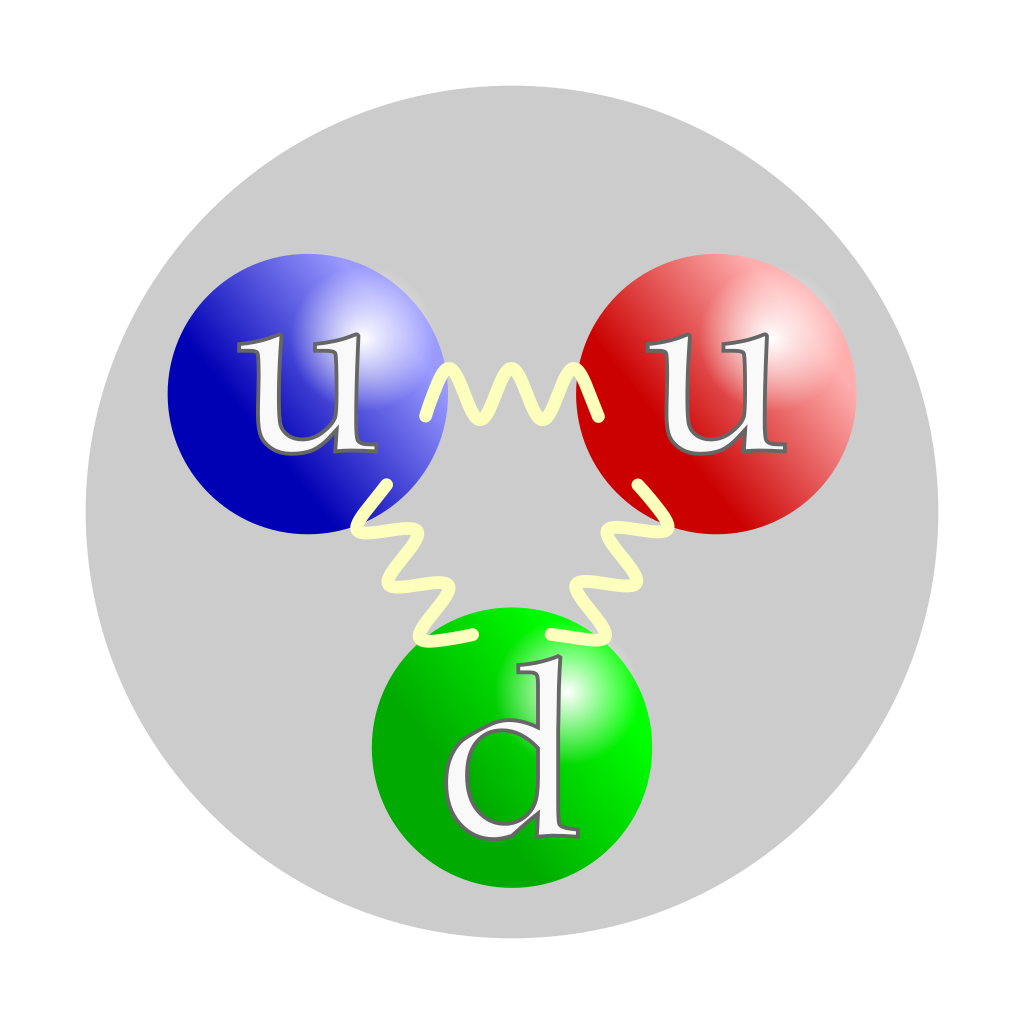
\includegraphics[width=100mm]{figures/protonQuarks.png}
  \caption{Quarks inside a proton.
    Labelled u for up and d for down}
  \label{protonQuarks}
\end{figure}

Further confirmation of the quark model came from the discovery of additional types of quarks and the development of Quantum Chromodynamics (QCD).
QCD provided a comprehensive framework for understanding how quarks are bound together.

Today, quarks are understood to be fundamental constituents of matter, forming the building blocks of protons, neutrons, and other hadrons (Composite subatomic particles that are made up of at least 2 quarks).

We have so far discovered 6 flavors of quarks -- up (\(u\)), down (\(d\)), charm (\(c\)), strange (\(s\)), top (\(t\)), and bottom (\(b\)).
Each flavor has different mass.
These masses and their interactions with other particles are crucial for the stability and properties of atomic nuclei.

\begin{table}[h!]
  % Could you please check if the numbers in the table are correct, I'm not 100 percent sure
  \centering
  \begin{tabular}{lrr}
    \toprule
    Quark Flavor & Approximate Mass (MeV/c\(^2\)) & Charge (e) \\
    \midrule
    Up (u)      & 2.2 - 3.0        & +\(\frac{2}{3}\) \\
    Down (d)    & 4.7 - 5.0        & -\(\frac{1}{3}\) \\
    Strange (s) & 95 - 105         & -\(\frac{1}{3}\) \\
    Charm (c)   & 1270 - 1720      & +\(\frac{2}{3}\) \\
    Bottom (b)  & 4180 - 4380      & -\(\frac{1}{3}\) \\
    Top (t)     & 172000 - 173000  & +\(\frac{2}{3}\) \\
    \bottomrule
  \end{tabular}
  \caption{Quark Flavors and Their Approximate Masses}
  \label{quarkMass}
\end{table}

Quarks carry fractional electric charges.
For instance, up quarks have a charge of \(+\frac{2}{3}\) e, while down quarks have a charge of \(-\frac{1}{3}\) e, where e is the elementary charge.
This fractional charge is essential for the charge balance in particles such as protons and neutrons.

Quarks are never found in isolation due to a phenomenon known as confinement.
They are always confined within larger particles called hadrons.

Quarks have a property called color charge, analogous to electric charge but related to the strong force.
There are three types of color charges: red, green, and blue.
The strong interaction, which is described by QCD, ensures that particles made of quarks are color-neutral.

For each quark flavor, there exists a corresponding antiquark with the opposite charge.
Antiquarks can combine with quarks to form mesons, another category of hadrons.



% \subsection{The Strong Force}

Having gone over what quarks are, the interesting question to ponder is why do quarks stay together to form hadrons?
Fundamentally, why can they not exist by themselves in a stable configuration?
The answer to both of these questions is the strong force.

It is a fundamental aspect of QCD, which is the theory describing the interactions of quarks and gluons.
Gluons are a massless particle that mediates the strong force and is part of the standard model.

The strong force is characterized by its incredibly short range but immense strength.
It operates effectively only at distances on the order of femtometers (1 fm = \(10^{-15}\) meters).

One of the key features of the strong force is quark confinement, which means that quarks are never found in isolation.
They are always bound within larger particles called hadrons.
This is due to the nature of the strong force, which becomes stronger as quarks move farther apart.
The potential energy associated with the strong force increases with distance, effectively confining quarks within hadrons.

The QCD Lagrangian, describes the strong force

\begin{align}
  \mathcal{L}_{\text{QCD}} &= -\frac{1}{4} F_{\mu\nu}^a F^{\mu\nu a} + \bar{\psi}_i (i \gamma^\mu D_\mu - m_i) \psi_i,
\end{align}

where \( F_{\mu\nu}^a \) is the field strength tensor for the gluon fields, \( \psi_i \) represents the quark fields, \( \gamma^\mu \) are the gamma matrices, and \( D_\mu \) is the covariant derivative that includes the gluon interaction.
The term \( -\frac{1}{4} F_{\mu\nu}^a F^{\mu\nu a} \) describes the dynamics of the gluon fields, and \( \bar{\psi}_i (i \gamma^\mu D_\mu - m_i) \psi_i \) describes the interaction between quarks and the gluon field.

Another fascinating property of the strong force is asymptotic freedom, which means that quarks interact more weakly at shorter distances.
This phenomenon is described by the running of the strong coupling constant \( \alpha_s \), which decreases as quarks come closer together:

\begin{align}
  \alpha_s(Q^2) &= \frac{g^2(Q^2)}{4 \pi},
\end{align}

where \( g(Q^2) \) is the running coupling constant that depends on the energy scale \( Q^2 \).
At high energies (short distances), \( \alpha_s \) becomes smaller, indicating weaker interactions between quarks.
Conversely, at low energies (larger distances), \( \alpha_s \) grows larger, leading to stronger interactions and quark confinement.

In practice, the strong force is responsible for the internal structure of hadrons.
The force between these quarks is mediated by gluons, which continuously exchange color charge and bind the quarks together in a stable configuration.
The interaction between quarks within hadrons can be described by the potential:

\begin{align}
  V(r) &= -\frac{4}{3} \frac{\alpha_s}{r},
\end{align}

where \( \alpha_s \) is the strong coupling constant and \( r \) is the distance between quarks.
This potential is known as the Cornell potential and illustrates how the force increases as quarks move further apart.



\subsection{Electroweak Theory}

Moving on to the other fundamental forces,  the combination of electromagnetism  and the weak force into one consistent theory  was monumental in pushing physics forward.The journey towards electroweak unification began with the discovery of the weak force, a crucial interaction responsible for processes like beta decay.
Early experiments revealed that the weak force was much weaker than electromagnetism and had a very short range.
It was eventually understood that the weak force and electromagnetism were manifestations of a more fundamental interaction.

In the 1970s, Sheldon Glashow, Abdus Salam, and Steven Weinberg formulated the electroweak theory, which successfully unified these two interactions into a single theoretical framework.
Their theory predicted the existence of the W and Z bosons, which mediate the weak force.
The electroweak theory is based on the gauge symmetry group $SU(2)_L \times U(1)_Y$.

The Lagrangian for the electroweak interaction can be written as

\begin{align}
\mathcal{L}_{\text{EW}} &= -\frac{1}{4} W^i_{\mu \nu} W^{i \mu \nu} - \frac{1}{4} B_{\mu \nu} B^{\mu \nu} \\
&\quad + \frac{1}{2} m_W^2 W^i_\mu W^{i \mu} + \frac{1}{2} m_Z^2 Z_\mu Z^\mu \\
&\quad - \frac{g}{2} \left( \bar{\psi}_L \gamma^\mu \frac{\tau^i}{2} W^i_\mu \psi_L \right) \\
&\quad - \frac{g'}{2} \left( \bar{\psi}_L \gamma^\mu Y \psi_L B_\mu \right) \\
&\quad - \frac{g}{2} \left( \bar{\psi}_R \gamma^\mu \frac{\tau^i}{2} W^i_\mu \psi_R \right) \\
&\quad - \frac{g'}{2} \left( \bar{\psi}_R \gamma^\mu Y \psi_R B_\mu \right) \\
&\quad + \frac{g}{2 \cos \theta_W} \left( \bar{\psi}_L \gamma^\mu \frac{\tau^i}{2} W^i_\mu \psi_L \right) \\
&\quad + \frac{g}{2 \cos \theta_W} \left( \bar{\psi}_L \gamma^\mu \frac{\tau^i}{2} Z_\mu \psi_L \right).
\end{align}

Where $W^i_{\mu \nu}$ represents the field strength tensor for the $SU(2)_L$ gauge bosons, $B_{\mu \nu}$ is the field strength tensor for the $U(1)_Y$ gauge boson, $m_W$ and $m_Z$ are the masses of the $W$ and $Z$ bosons respectively, $g$ is the $SU(2)_L$ gauge coupling constant, $g'$ is the $U(1)_Y$ gauge coupling constant, $\psi_L$ and $\psi_R$ denote the left- and right-handed fermion fields, $\tau^i$ are the Pauli matrices corresponding to the $SU(2)_L$ symmetry, $Y$ represents the hypercharge of the fermion fields, and $\theta_W$ is the Weinberg angle.



The electroweak theory successfully predicted the masses of the $W$ and $Z$ bosons, which were experimentally confirmed in 1983 at CERN.
The $W$ bosons ($W^+$ and $W^-$) mediate charged current interactions, while the $Z$ boson mediates neutral current interactions.

The path to the electroweak theory was marked by significant experimental and theoretical advances.
In the 1930s, the discovery of the muon by Carl Anderson and Seth Neddermeyer introduced the idea that there were particles beyond the electron.
Muons were soon identified as heavier cousins of electrons, leading to the development of the concept of lepton family.

In the 1970s, the discovery of the tau lepton, a particle even heavier than the muon, further expanded the lepton family.
The tau lepton, discovered by Martin Perl and collaborators in 1975, was crucial in validating the electroweak theory.
The existence of three generations of leptons (electron, muon, and tau) and their associated neutrinos was essential for the theory's development.

The electroweak unification also prompted the search for new particles, such as the Higgs boson, responsible for giving mass to the gauge bosons.
The discovery of the Higgs boson at the Large Hadron Collider in 2012 was a triumph for the Standard Model and confirmed the last missing piece of the electroweak theory.





\subsection{neutrino}\
Okay!

The stage has been set!

Time for our stars --the neutrinos-- to make an appearence.

The story begins in the 1930s with Wolfgang Pauli, who first proposed the existence of neutrinos to solve a pressing problem in the field of beta decay.
He addressed the puzzle of the missing energy in beta decay experiments.
Beta decay is a process where a neutron decays into a proton, an electron, and an electron antineutrino:

\[
  n \rightarrow p + e^- + \bar{\nu}_e
\]

where \( n \) is the neutron, \( p \) is the proton, \( e^- \) is the electron, and \( \bar{\nu}_e \) is the electron antineutrino.
The problem was that the energy of the emitted beta particle (electron) and the proton did not add up to the total energy of the decaying neutron, leading to what seemed like a violation of energy conservation.

To deal with this, Pauli proposed the existence of a new, neutral particle that carried away the missing energy.
\footnote{He called this hypothetical particle the "neutron" (not to be confused with the neutron in the nucleus), but it was later renamed the "neutrino" by Enrico Fermi in 1934.}
Fermi incorporated the neutrino into his theory of beta decay, which became known as Fermi's theory of beta decay.
His theory elegantly explained the conservation of energy and angular momentum in beta decay processes.

The neutrino, denoted by \( \nu \), is a nearly massless and electrically neutral particle.
The interaction of neutrinos is governed by the weak force

For many years, neutrinos were a theoretical construct until they were finally observed experimentally by Clyde Cowan and Frederick Reines in 1956.
Their detection was achieved by capturing neutrinos emitted from a nuclear reactor and observing their interactions with a detector filled with water and cadmium chloride.

The weak interaction is described by the exchange of W and Z bosons, which mediate processes like beta decay.

The 1960s introduced a new chapter with the discovery of the muon neutrino, $\nu_\mu$.
The experiment conducted by the Brookhaven National Laboratory used a beam of pions, which decay into muons and muon neutrinos:

\begin{align}
  \pi^+ \rightarrow \mu^+ + \nu_\mu
\end{align}

Here, $\pi^+$ is the positively charged pion, $\mu^+$ is the muon, and $\nu_\mu$ is the muon neutrino.
In 1962, the collaboration led by Martin LPerl and his team at the Stanford Linear Accelerator Center (SLAC) confirmed the existence of the muon neutrino by observing interactions consistent with $\nu_\mu$.

The next breakthrough in neutrino physics came in 1975 with the discovery of the tau neutrino, $\nu_\tau$.
The relevant interaction can be expressed as:

\begin{align}
  \tau^+ \rightarrow \nu_\tau + \ell^+
\end{align}

where $\tau^+$ is the positively charged tau particle, $\nu_\tau$ is the tau neutrino, and $\ell^+$ represents a lepton like a positron.
The detection of the tau neutrino was more challenging due to its lower production rates and the complexity of distinguishing it from other neutrinos.
These discoveries not only confirmed the existence of the muon and tau neutrinos but also led to the realization of the three-flavor neutrino model in the Standard Model.



\subsection{Neutrino Mass Ordering}

In the early days of neutrino physics, the Standard Model treated neutrinos as massless particles but experimentally we know that they have some amount of mass.
Just a very tiny amount.
Not only do we not really know the masses of the neutrinos, the ordering of their masses is still an open question.

For the mass ordering of neutrinos, we need to delve into the concept of neutrino mass eigenstates and flavor eigenstates.
Neutrinos are produced and detected in flavor eigenstates (denoted by $\nu_e$, $\nu_\mu$, and $\nu_\tau$), but they propagate as mass eigenstates ($\nu_1$, $\nu_2$, and $\nu_3$).
The relationship between these states is governed by the PMNS (Pontecorvo-Maki-Nakagawa-Sakata) matrix \cite{PMNS_matrix}, which can be written as:

\begin{align}
  \begin{pmatrix}
    \nu_e \\
    \nu_\mu \\
    \nu_\tau
  \end{pmatrix}
  =
  \begin{pmatrix}
    U_{e1} & U_{e2} & U_{e3} \\
    U_{\mu1} & U_{\mu2} & U_{\mu3} \\
    U_{\tau1} & U_{\tau2} & U_{\tau3}
  \end{pmatrix}
  \begin{pmatrix}
    \nu_1 \\
    \nu_2 \\
    \nu_3
  \end{pmatrix}
\end{align}

The mass eigenstates $\nu_1$, $\nu_2$, and $\nu_3$ have different masses, but their exact ordering is not yet definitively known \cite{De_Angelis_Pimenta_2018}.
There are two possible orderings for these masses:

Normal Ordering (NO): In this scenario, the masses of the neutrinos are ordered as \( m_1 < m_2 < m_3 \).
This implies that the third eigenstate, $\nu_3$, has the highest mass.
The mass differences between these states are described by:

\begin{align}
  \Delta m_{21}^2 &= m_2^2 - m_1^2 \\
  \Delta m_{32}^2 &= m_3^2 - m_2^2 \\
  \Delta m_{31}^2 &= m_3^2 - m_1^2
\end{align}

Inverted Ordering (IO): Here, the masses are ordered as \( m_3 < m_1 < m_2 \).
In this case, the lightest eigenstate is $\nu_3$.
The corresponding mass differences are:

\begin{align}
  \Delta m_{21}^2 &= m_2^2 - m_1^2 \\
  \Delta m_{32}^2 &= m_2^2 - m_3^2 \\
  \Delta m_{31}^2 &= m_1^2 - m_3^2
\end{align}

Determining the correct mass ordering is essential for understanding the properties of neutrinos and has profound implications for cosmology and particle physics.


\subsection{Neutrino Oscillations}

Neutrino oscillation is a quantum phenomenon whereby a neutrino created with a specific lepton flavor can change into another flavor as it propagates through space.
This behavior is a direct consequence of the fact that neutrinos have mass and the flavor eigenstates \cite{Barger_Marfatia_Whisnant_2012}.


The flavor states \(\nu_\alpha\) (\(\alpha = e, \mu, \tau\)) are related to the mass states \(\nu_i\) (\(i = 1, 2, 3\)) through a unitary transformation.
This transformation can be expressed as:

\begin{align}
|\nu_\alpha\rangle &= \sum_{i} U_{\alpha i} |\nu_i\rangle,
\end{align}

where \(U_{\alpha i}\) are elements of the PMNS matrix, which is a unitary matrix describing the mixing between the flavor and mass eigenstates.

When a neutrino is produced in a flavor eigenstate \cite{Cohen_Glashow_Ligeti_2009}, it propagates as a superposition of mass eigenstates\cite{PhysRevD.97.072009}.
If we denote the neutrino state produced at \(t = 0\) as \(|\nu_\alpha\rangle\), its time evolution in terms of the mass eigenstates is given by:

\begin{align}
|\nu_\alpha(t)\rangle &= \sum_{i} U_{\alpha i} e^{-i E_i t} |\nu_i\rangle,
\end{align}

where \(E_i\) is the energy of the mass eigenstate \(\nu_i\), and \(t\) is the time of propagation.

The probability of detecting a neutrino of flavor \(\beta\) after a time \(t\) is given by the squared modulus of the amplitude \cite{Barger_Marfatia_Whisnant_2012}:

\begin{align}
P(\nu_\alpha \to \nu_\beta; t) &= \left| \langle \nu_\beta | \nu_\alpha(t) \rangle \right|^2 \\
&= \left| \sum_{i} U_{\beta i}^* U_{\alpha i} e^{-i E_i t} \right|^2.
\end{align}

Assuming the mass differences between the neutrino mass eigenstates are small compared to their energies, and using the approximation \(E_i \approx E - \frac{m_i^2}{2E}\), we can simplify the expression for the oscillation probability.
The oscillation probability for a two-flavor scenario (\(\alpha\) and \(\beta\)) is given by:

\begin{align}
P(\nu_\alpha \to \nu_\beta; L) &= \sin^2(2\theta) \sin^2\left(\frac{\Delta m^2 L}{4 E}\right),
\end{align}

where \(\theta\) is the mixing angle between the two flavors, \(\Delta m^2 = m_2^2 - m_1^2\) is the mass-squared difference, \(L\) is the distance traveled by the neutrino, and \(E\) is the neutrino's energy.


\subsection{Dirac Vs MAJORANA Neutrinos}

To understand the nature of neutrino masses, it is crucial to delve into two different types of neutrinos; Dirac and Majorana.
So a new model was required to explain these discrepancies, and in comes Dirac.
Dirac, in 1928, extended his theory to include neutrinos, proposing that they were Dirac fermions.
According to Dirac's theory, neutrinos have distinct antiparticles, and their masses arise from the Higgs mechanism, similar to other fermions.
In the Dirac framework, the Lagrangian for neutrinos can be written as:

\begin{align}
  \mathcal{L}_{\text{Dirac}} &= \bar{\nu}_L (i\gamma^\mu \partial_\mu - m_\nu) \nu_L + \text{h.c.},
\end{align}

where \(\nu_L\) denotes the left-handed neutrino field, \(\bar{\nu}_L\) its Dirac adjoint, and \(m_\nu\) is the Dirac mass term.
\(\nu_L\) and its antiparticle \(\bar{\nu}_L\) are distinct entities.

Then comes Majorana, who proposed in 1937 a different theory to account for neutrino masses.
Majorana suggested that neutrinos could be their own antiparticles, which leads to the Majorana condition.
In this framework, neutrinos are described by Majorana fermions.
The Majorana Lagrangian is given by:

\begin{align}
  \mathcal{L}_{\text{Majorana}} &= \frac{1}{2} \bar{\nu}_L^c (i\gamma^\mu \partial_\mu - m_\nu) \nu_L + \text{h.c.},
\end{align}

where \(\nu_L^c\) is the charge-conjugated field of \(\nu_L\).
The Majorana mass term explicitly breaks the lepton number conservation, which is a key difference from the Dirac case.
Lepton number conservation is the principle that the total number of leptons minus antileptons remains constant in a physical process.
Majorana neutrinos are their own antiparticles, and their mass term is of the form:

\begin{align}
  \mathcal{L}_{\text{Majorana mass}} &= -\frac{1}{2} m_\nu (\nu_L^T C \nu_L + \text{h.c.}),
\end{align}

where \(C\) is the charge-conjugation matrix.


The actual nature of neutrino masses—whether Dirac or Majorana—has significant implications for our understanding of fundamental particles and the symmetries of the universe.


